\documentclass[12pt]{article}
\usepackage[utf8]{inputenc}
\usepackage{alphabeta}
\usepackage[colorinlistoftodos]{todonotes}
\usepackage{graphicx,lipsum}
\usepackage{enumerate}
\usepackage{xcolor}
\usepackage[hidelinks]{hyperref}
\usepackage{multirow}
\graphicspath{ {./images/} }
\usepackage{ltablex,booktabs}
\usepackage{tikz}
\usepackage{multicol}
\usepackage{subcaption} 
\tikzstyle{mybox} = [draw=black, very thick, rectangle, inner xsep=7pt, inner ysep=7pt, minimum height=50mm, minimum width=50mm, text width=50mm-2*\pgfkeysvalueof{/pgf/inner xsep}]
\usepackage{copyrightbox}
%%%% figure-copyright
\usepackage{url}
\usepackage{placeins}
\usepackage{hyperref}
\usepackage{ltablex,booktabs}
\hypersetup{
	colorlinks=true,
	%linkcolor=blue,
	filecolor=magenta,      
	urlcolor=blue,
}
\setlength\parindent{0pt}
\begin{document}
	
	\begin{titlepage}
		
		\begin{figure}[h!]
			\centering
			
\includegraphics[width=10cm,height=3cm]{uni}
		\end{figure}
		
		\begin{center}
			\vspace*{0.2cm}

			\Large
			Stack Overflow Tag Network
			\vspace{0.5cm}
			\centering
			
\includegraphics[width=15cm,height=3cm]{stackoverflowlogo}
			\vfill
			\Large
			Network Analysis\\
			Supervisor Professor: Dimitrios Pournarakis
			
			\vspace{1.5cm}
			
			\textbf \small {Rafaila Galanopoulou 8160018}
			
			\vspace{2.5cm}
			\centering
			
		\end{center}
	\end{titlepage}
	
	\clearpage
	\hypersetup{linkcolor=black}
	\tableofcontents
	\clearpage
\section{Idea}
	Searching for a network dataset that would be interesting to analyse, I found this network (edges and nodes) of Stack Overflow tags based on Developer Stories. "Stack Overflow is a question and answer site for professional and enthusiast programmers. It is a privately held website, the flagship site of the Stack Exchange Network, created in 2008 by Jeff Atwood and Joel Spolsky. It features questions and answers on a wide range of topics in computer programming" \href{https://en.wikipedia.org/wiki/Stack_Overflow}{Wikipedia}. \\
	According to its creators the data team at Stack Overflow, they spend a lot of their time and energy thinking about tech ecosystems and how technologies are related to each other. They discover that a way to get at this idea of relationships between technologies is tag correlations, how often technology tags at Stack Overflow appear together relative to how often they appear separately. One place we see developers using tags at Stack Overflow is on their Developer Stories, or professional profiles/CVs/resumes. If we are interested in how technologies are connected and how they are used together, developers' own descriptions of their work and careers is a great place to get that.\\
	Each month, about 50 million people visit Stack Overflow to learn, share, and build their careers. We estimate that 21 million of these people are professional developers and university-level students. The majority of our survey respondents this year were people who said they are professional developers or who code sometimes as part of their work, or are students preparing for such a career. About 4\% of respondents code as a hobby but not as a profession, and just under 2\% of respondents used to be professional developers but no longer are. According to the  \href{https://insights.stackoverflow.com/survey/2019#key-resultsl}{Stack Overflow Survey}.
		\begin{figure}[ht]
			\centering
		
\includegraphics[width=12cm,height=10cm]{stackoverflowfun}
		\caption{The role of Stack Overflow in our lives\\
		\tiny \href{https://www.reddit.com/r/ProgrammerHumor/comments/bvx7vv/stackoverflow_is_for_eaveryone/}{Source}}
	\end{figure}
	\FloatBarrier
	The main reason that I selected this worldwide known and used platform network stems from my recent search for an internship placement. It was very stressful to search 24/7 what is on high demand in the market workplace and if my studies are enough in order to start a career. As a junior level developer, I found quite interesting to see all the relationships between in-trend technologies but most importantly to answer the question "Which are the prerequisite technological background of learning each technology?".\\
	The Python notebooks created for Data Preprocessing and Network Analysis are available \href{https://github.com/Rafaila98/Stack-Overflow-Tag-Network}{here}. 
	
\section{Dataset}

	\subsection{Source}
		The dataset selected for the Network Analysis is the Stack Overflow Tag Network and can be found in \href{https://www.kaggle.com/stackoverflow/stack-overflow-tag-network}{Kaggle}.
	
	\subsection{Data Overview}
		The dataset represents a network of technology tags from Developer Stories on the Stack Overflow online developer community website.\\
		It is consisted the following two files:
		\begin{itemize}
			\item \underline{stack\_network\_edges.csv } contains links of the network, the source and target tech tags plus the value of the the link between each pair. A graph consists of nodes and edges. In this case the nodes are the tags that appear in a developer's profile in stackoverflow "Developer Stories". If two tags appear on the same profile there's a tag between them. \\
			The dataset include only a subset of tags used on Developer Stories, tags that were used by at least 0.5\% of users and were correlated with another tag with a correlation coefficient above 0.1. This means that very sparsely used tags and tags that are not used with other tags were filtered out.\\
			This file also includes the links of the network in 3 columns: 
			\begin{itemize}
				\item Source tech tags 
				\item Target tech tags 
				\item Value of the the link between each pair, which means how correlated those two tags are (correlation coefficient * 100)
			\end{itemize}
			\item \underline{stack\_network\_nodes.csv} contains nodes of the network, the name of each node, which group that node belongs to (calculated via a cluster walktrap), and a node size based on how often that technology tag is used.\\
			This file also includes the links of the network in 3 columns: 
			\begin{itemize}
				\item name of tech tags 
				\item group in which each node belongs to (calculated via a cluster walktrap)
				\item nodesize which is proportional to how many developers have that tag in their developer story profile
			\end{itemize}
		\end{itemize}
	
	\subsection{Data Preprocessing}
		The dataset was already cleaned so no null or missing values exist and, thus, no cleaning was necessary. Although using Python, I checked it, as it seems below.\\
		\begin{figure}[ht]
			\begin{subfigure}[b]{0.24\textwidth}
				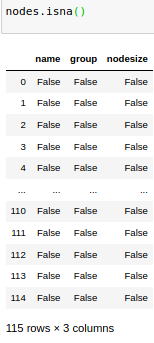
\includegraphics[width=\textwidth]{nodesnan}
				\caption{nodes.csv\\
				\tiny {It would be True if there were any NaN values}}
				\label{fig:1}
			\end{subfigure}
			\hfill 
			\begin{subfigure}[b]{0.282\textwidth}
				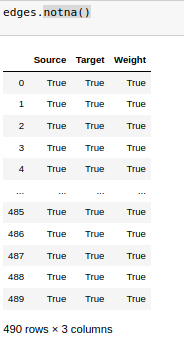
\includegraphics[width=\textwidth]{edgessnan}
				\caption{edges.csv\\
				\tiny {It would be False if there were any NaN values}}
				\label{fig:2}
			\end{subfigure}
		\end{figure}
		\FloatBarrier
		\subsubsection{Nodes Table}
			In the original dataset the Id of each tag was its own name. In order to be correctly represented as a graph in Gephi according to the \href{https://youtu.be/HJ4Hcq3YX4k}{tutorial}, I created a unique Id for each tag. 
			\begin{figure}[ht]
				\begin{subfigure}[b]{0.5\textwidth}
					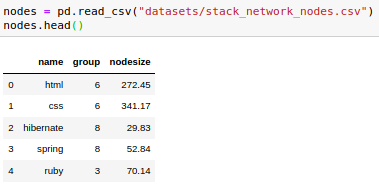
\includegraphics[width=\textwidth,height=5cm]{nodesinit}
					\caption{initial nodes table}
					\label{fig:1}
				\end{subfigure}
				\hfill 
				\begin{subfigure}[b]{0.4\textwidth}
					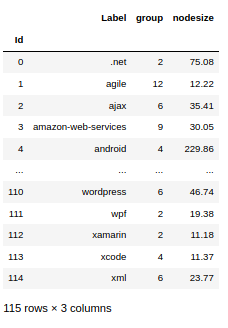
\includegraphics[width=\textwidth,height=7cm]{nodesfinal}
					\caption{final nodes table}
					\label{fig:2}
				\end{subfigure}
			\end{figure}
		\FloatBarrier
		
		\subsubsection{Edges Table}
			In this table, a new Id column was added, which was also the index of the table, and the column name renamed as Label.
			\begin{figure}[ht]
				\begin{subfigure}[b]{0.5\textwidth}
					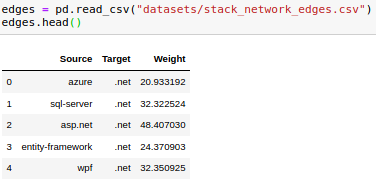
\includegraphics[width=\textwidth,height=5cm]{edgesinit}
					\caption{initial edges table}
					\label{fig:1}
				\end{subfigure}
				\hfill 
				\begin{subfigure}[b]{0.4\textwidth}
					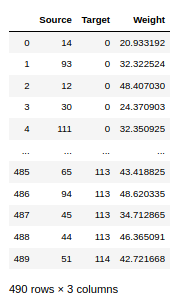
\includegraphics[width=\textwidth,height=7cm]{edgesfinal}
					\caption{final edges  table}
					\label{fig:2}
				\end{subfigure}
			\end{figure}
		\FloatBarrier
	
	\section{Graph Representation}
		The first representation of the graph is according to dataset raw data. That means that each group has its own colour and each node is sized according to nodesize variable. The problem with this graph is that it is undirected and the Source \& Target columns are not totally exploited.  
			\begin{figure}[ht]
					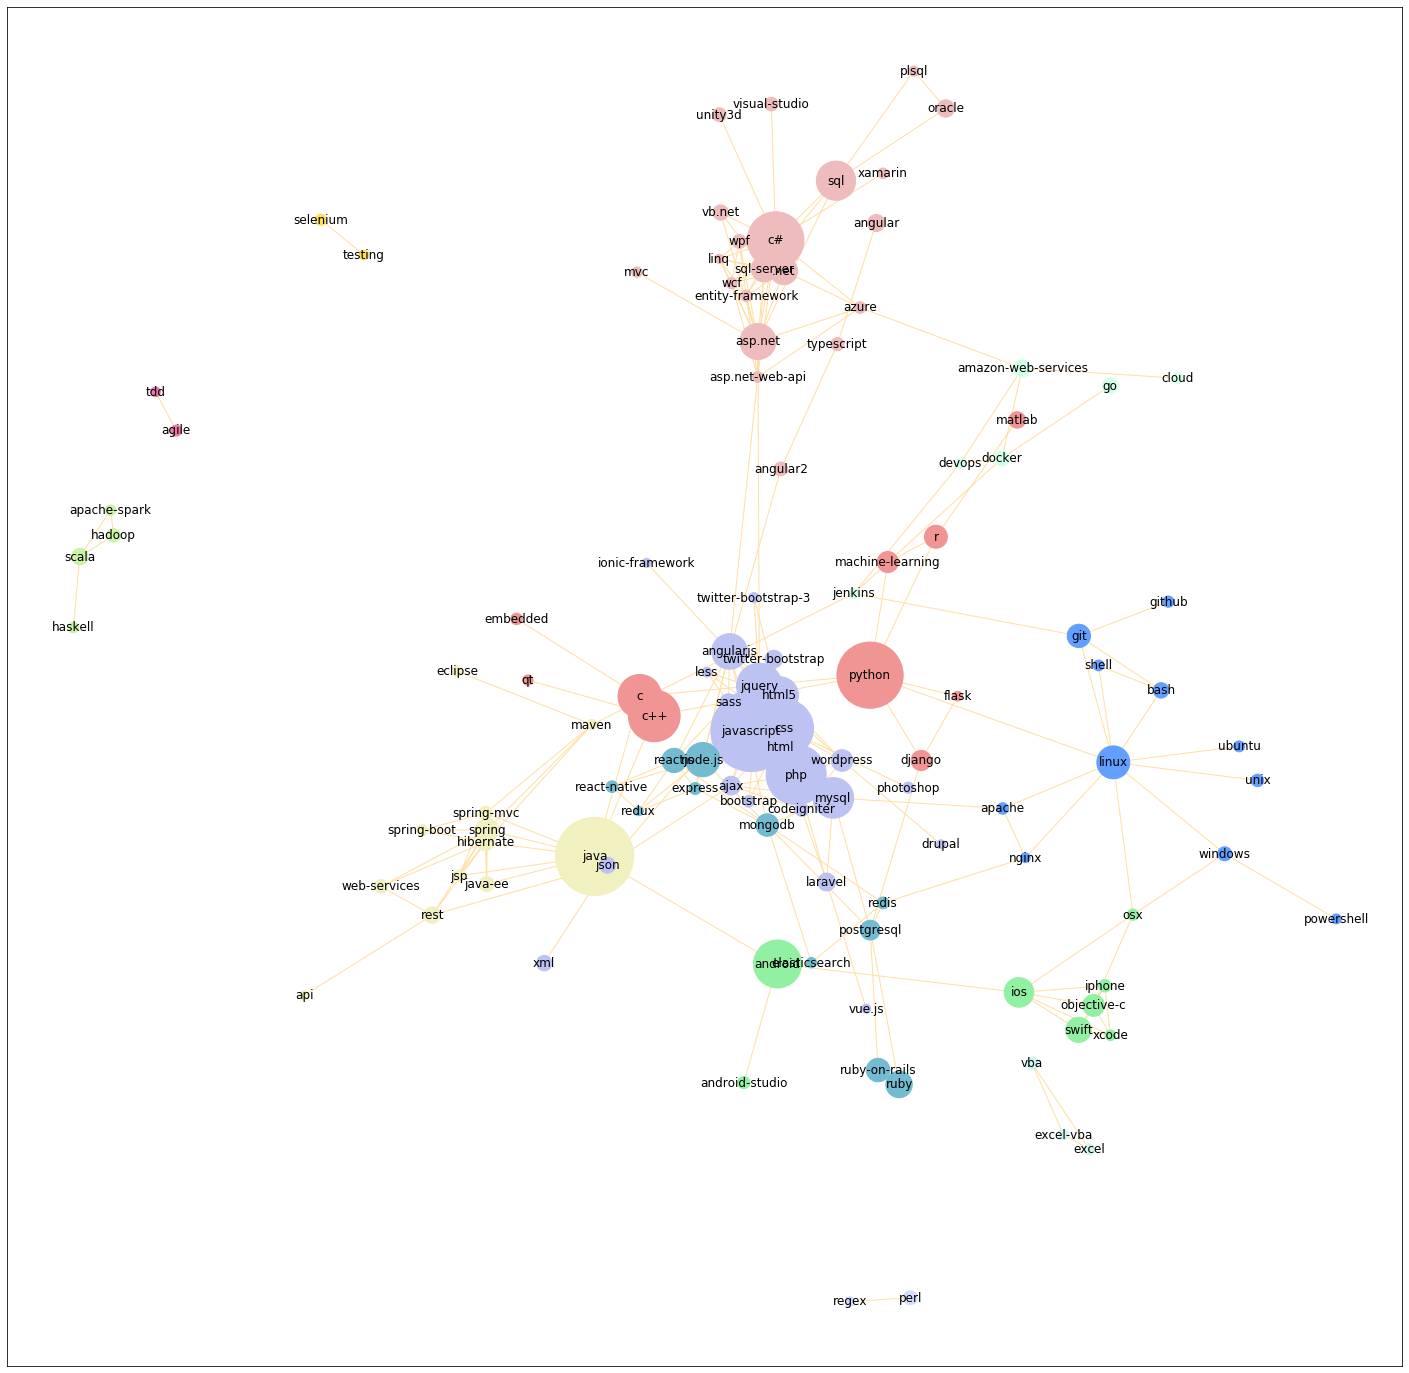
\includegraphics[width=17cm,height=20cm]{index}
					\caption{Network}
			\end{figure}
		\FloatBarrier
		The two following representations was made with \href{https://gephi.org/}{Gephi}.\\
		The network below has different colours for each of 14 group that exist by default in the dataset. 
		\begin{figure}[ht]
			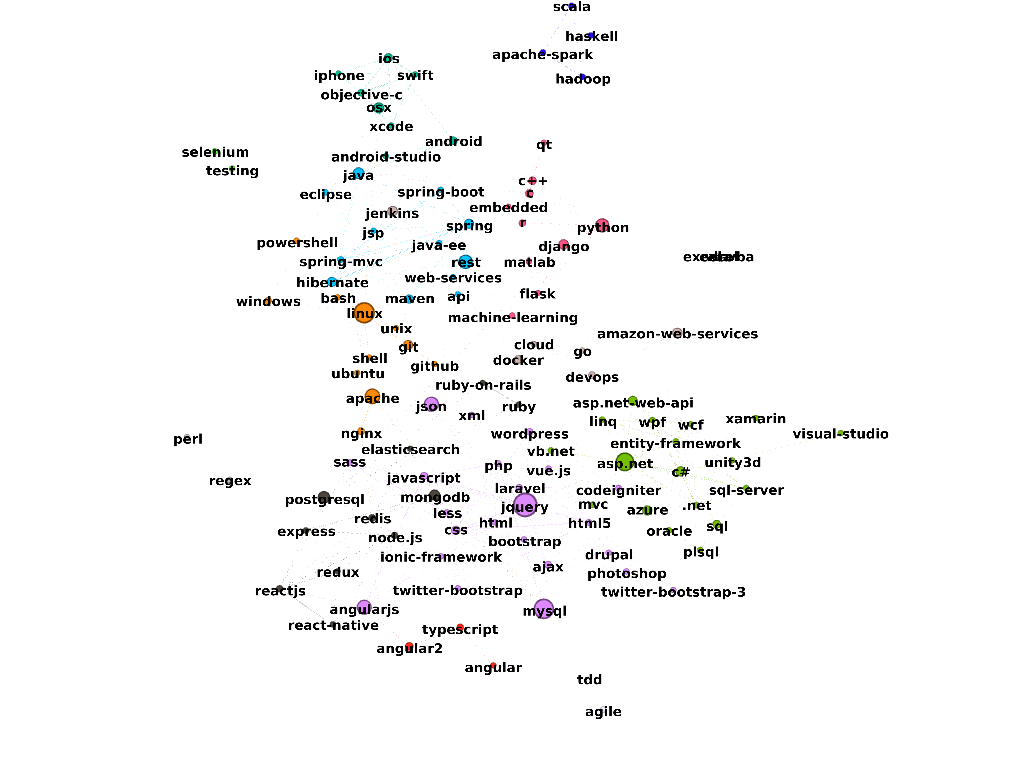
\includegraphics[width=17cm,height=14cm]{network}
			\caption{Network with Gephi 1st version}
		\end{figure}
		\FloatBarrier
		\clearpage 
		The network below has different different colours for each of 14 group, the edges have ranking based on their Weight, the size of nodes and their labels' font size have ranking according to the nodesize variable that exist by default in the dataset. 
		\begin{figure}[ht]
			\centering
			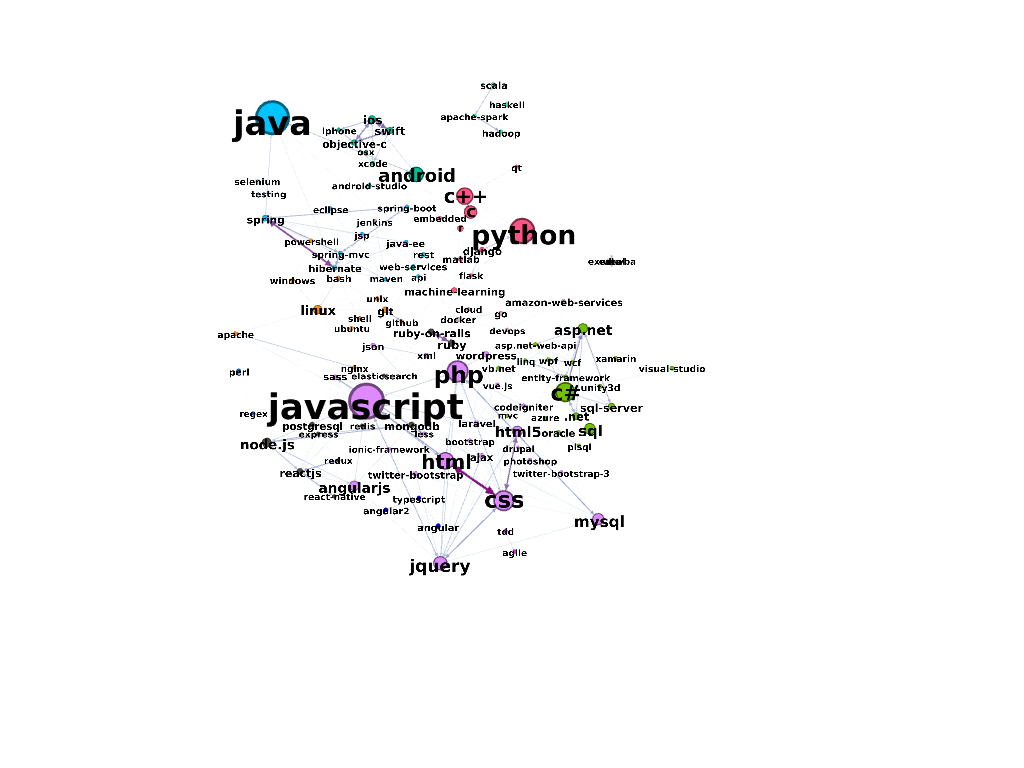
\includegraphics[width=20cm,height=14cm]{nodesize2}
			\caption{Network with Gephi 2nd version}
		\end{figure}
		\FloatBarrier
	
	\section{Basic Topological Properties}
		\begin{itemize}
			\item Number of nodes: 115
			\item Number of edges: 490
			\item Network diameter: 10 which is the biggest shortest path connecting two nodes.
			\item Average shortest path: $4.5$ which means that two nodes have distance of $4.5$ between them approximately.
			\item Network Density: $0.0374$ , which means that is absolutely not a dense network for reasons being explicitly explained below. 
		\end{itemize}
		
	
   \section{Component Measures}
      According to the Connected Components report in Gephi, for this undirected network, there are 6 weakly connected components and 6 strongly connected components. More specifically in Gephi, as Appearance Ranking value for nodes of the network we choose the Component ID and the result is the following graph.  
      	\begin{figure}[ht]
	      	\centering
	      	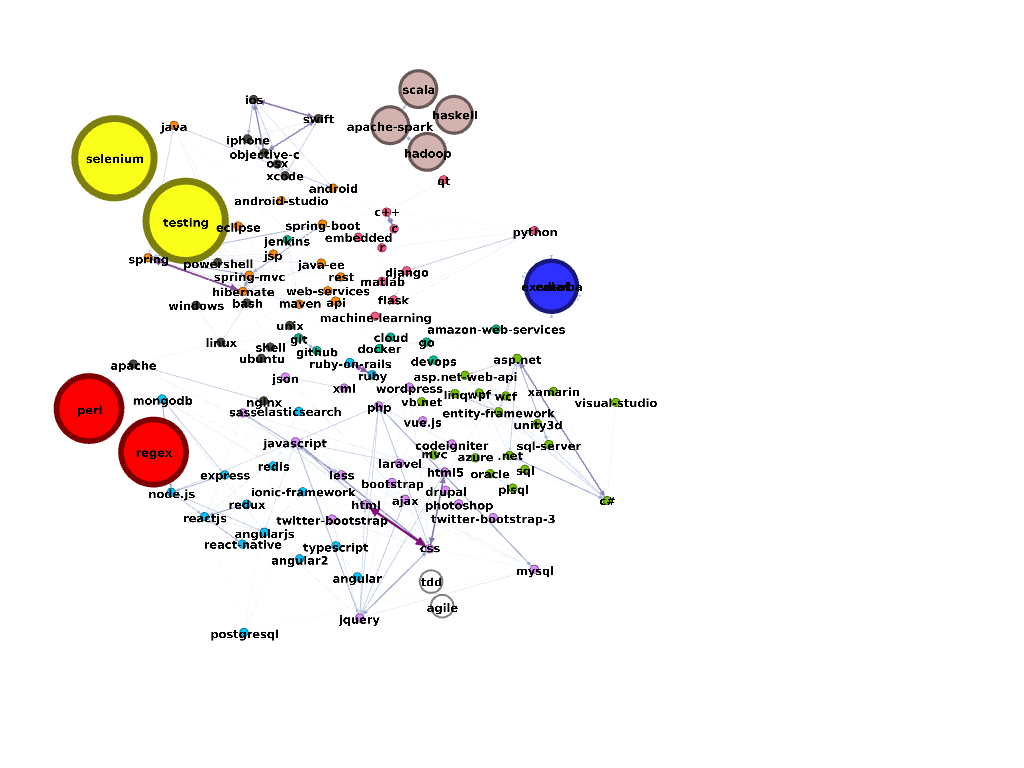
\includegraphics[width=20cm,height=10.5cm]{components}
	      	\caption{Components of the network}
      \end{figure}
      \FloatBarrier
      It is normal that regex and perl are one of the components, due to the fact that regural expressions are more usual in perl. Moreover, the blue circle on the right is all the excel nodes, which obviously has nothing in common with the rest nodes of the network. 
      
    \section{Degree Measures}
    	The average degree of this network is $4.2609$. The tag with the highest degree is jquery with $16$. 
   	 	\begin{figure}[ht]
    		\centering
    		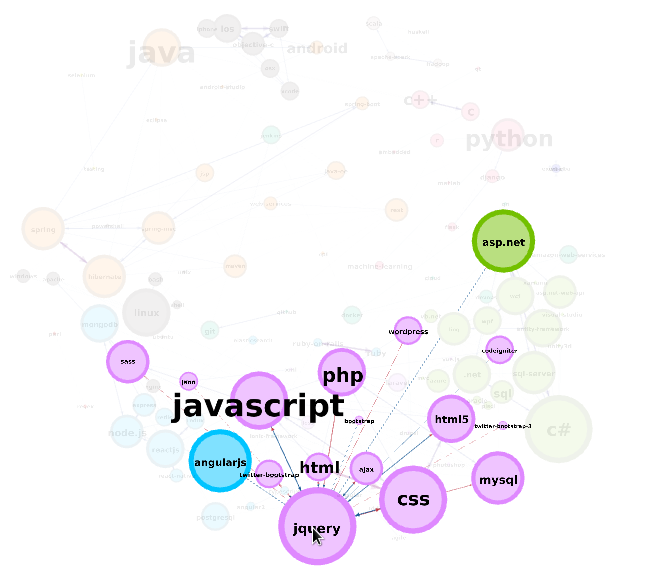
\includegraphics[width=15cm,height=10.5cm]{highestdegree}
    		\caption{Node with the highest degree}
    	\end{figure}
		 \FloatBarrier
	    The degree distribution shows us that most of the tags have degree $1$ and $3$.
	        \begin{figure}[ht]
		    	\centering
		    	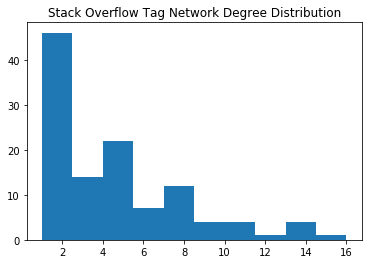
\includegraphics[width=7cm,height=5cm]{degreedistr}
		    	\caption{Node with the highest degree}
		    \end{figure}
		\FloatBarrier
		The average weighted degree is $148.995$, which is higher than average degree, because the weight of each link is considered. \\
		It is natural jquery to be the most connected node due to the fact that is a library for JavaScript, which is a broadly used and on high demand web development language. 
	
	\section{Centrality Measures}
		\subsection{Degree Centrality}
			The Degree Centrality shows how connected a node is. In this network the Degree Centrality shows how a tag (whether is a language or framework) is connected with all others tags and how all these technologies are finally connected. \\
			Top 10 tags with the highest degree are the followings:
			\begin{center}
				\begin{tabular}{ |c|c| } 
					\hline
					jquery & $16$  \\ 
					css & $14$ \\
					c\# & $14$ \\
					asp.net & $13$ \\
					angularjs & $13$ \\
					javascript &$12$ \\
					mysql & $11$ \\
					html5 & $10$ \\
					php & $10$ \\
					linux & $10$ \\
					\hline
				\end{tabular}
			\end{center}

		\subsection{Betweenness Centrality}
			Betweenness Centrality shows how important a node is in terms of connecting other nodes. In this case which tags are part of the shortest paths between two others and eventually we could say which technologies may be prerequisites of others.
			Top 10 tags with the highest betweenness centrality degree are the followings:
			\begin{center}
				\begin{tabular}{ |c|c| } 
					\hline
					jquery & $0.2555$  \\ 
					linux & $0.2084$ \\
					mysql & $0.1977$ \\
					asp.net & $0.1741$ \\
					apache & $0.1309$ \\
					json &$0.1232$ \\
					angularjs & $0.1229$ \\
					rest & $0.1137$ \\
					python & $0.1102$ \\
					postgresql & $0.0876$ \\
					\hline
				\end{tabular}
			\end{center} 
		Linux has the second highest betweenness centrality degree and that is because of being one of the most broadly used Operational Systems, especially in the developers community. There are daily developed and come in production new applets, plug-ins and other technologies compatible for Linux OS.
		
		\subsection{Closeness Centrality}
		The Closeness Centrality shows how close a node is to the centre of th network. This number is based on the length of the average shortest path between a tag and the rest tags of the network. \\
		Top 10 tags with the highest closeness centrality degree are the followings:
			\begin{center}
				\begin{tabular}{ |c|c| } 
					\hline
					jquery & $0.2896$  \\ 
					mysql & $0.2779$ \\
					ajax & $0.2586$ \\
					css & $0.2579$ \\
					javascript & $0.2571$ \\
					angularjs & $0.2571$ \\
					apache & $0.2549$ \\
					php & $0.2514$ \\
					html & $0.2472$ \\
					asp.net & $0.2465$\\
					\hline
				\end{tabular}
			\end{center} 
		Top 10 tags have the highest closeness centralities degrees are all connected with the most central node, which is jQuery, as we already mentioned. All are technologies (programming languages, frameworks etc.) which  are working complementary(html,css) or using jQuery to work (JavaScript).
		\subsection{Eigenvector Centrality}
			Eigenvector  centrality shows how much a node is connected to other important nodes in the network. It is a weighted degree centrality with a feedback boost for being connected with other important tags.\\
			Top 10 tags with the highest eigenvector centrality degree are the followings:
			\begin{center}
				\begin{tabular}{ |c|c| } 
					\hline
					jquery & $0.3658$  \\ 
					css & $0.3387$ \\
					javascript & $0.3256$ \\
					html5 & $0.2681$ \\
					php & $0.2653$ \\
					angularjs & $0.2652$ \\
					sass& $0.2521$ \\
					mysql & $0.2393$ \\
					twitter-bootstrap & $0.2071$\\
					html a& $0.2038$\\
					\hline
				\end{tabular}
			\end{center} 
		Technologies above concerns all those frameworks and languages which are using jQuery as a prerequisite to work correctly on the platform implemented. For example, twitter-bootstrap is the most popular HTML, CSS, and JS library in the world and require jQuery. 
		\subsection{PageRank Centrality}
			PageRank is a variant of Eigenvector Centrality but their main difference is that  the former accounts for link direction. Each tag in the network is assigned a score based on its indegree. These links are also weighted depending on the relative score of its originating node. 
			       \begin{figure}[ht]
						\centering
						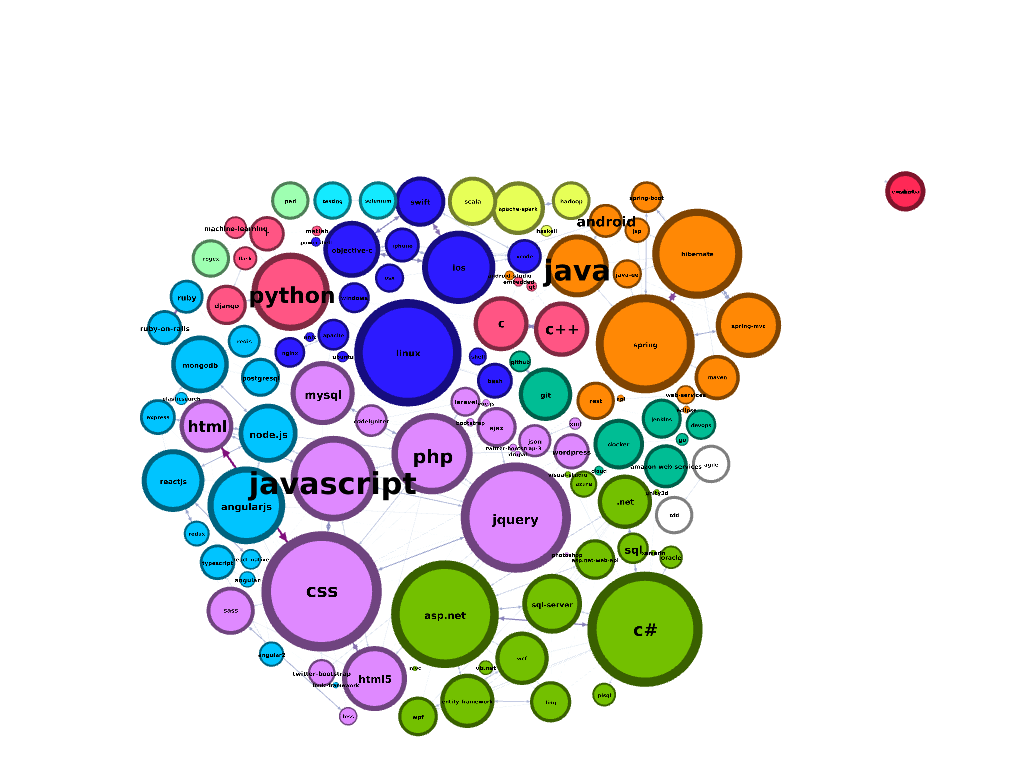
\includegraphics[width=10cm,height=7cm]{pagerank}
						\caption{PageRank Centrality Network}
				\end{figure}
			\FloatBarrier
			Network with size of each node according to pagerank centrality. The colours is according to which modularity class each node belongs to and fontsize of each label is based on nodesize default variable.
			
	\section{Clustering Effects}
		%The Average Clustering Coefficient is the mean value of individual coefficients
		The average clustering coefficient of this network is $0.615$, which means that there is 61.5\% possible that 2 tags be connected if there are connected to an A tag. \\
		\begin{figure}[ht]
			\centering
			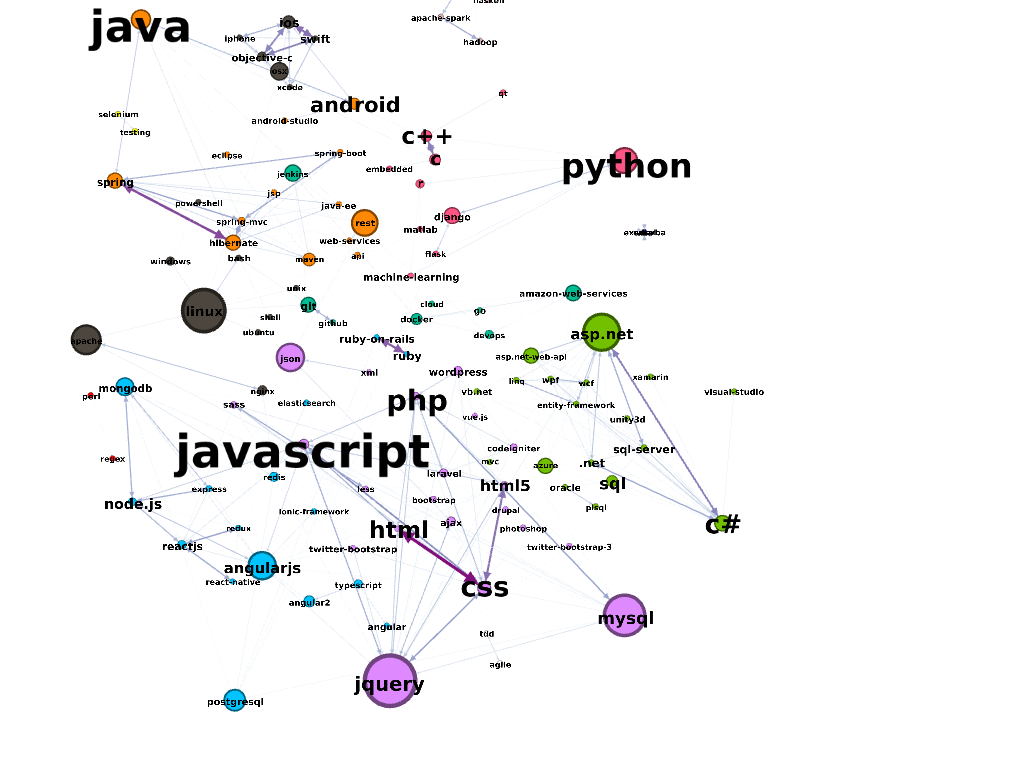
\includegraphics[width=10cm,height=7cm]{gephicluster}
			\caption{Cluster in Gephi}
		\end{figure}
		\FloatBarrier
		Triadic closure supposes that if two people know the same person, they are likely to know each other. If x is connected with both y and w, then y and w may very well know each other, completing a triangle in the visualization of three edges connecting x, y, and w. The number of these enclosed triangles in the network can be used to find clusters and communities of individuals that all know each other fairly well. One way to measure triadic closure is called clustering coefficient because of this clustering tendency, but it is also known as transitivity.Transitivity is the ratio of all triangles over all possible triangles. A possible triangle exists when one tag x knows two others (y and w). So transitivity, like density, expresses how interconnected a graph is in terms of a ratio of actual over possible connections.
		Triadic closure of this network is $0.4871$\\
		Also like density, transitivity is scaled from 0 to 1, and you can see that the network’s transitivity is about 0.487092, somewhat higher than its 0.037376 density. Because the graph is not very dense, there are fewer possible triangles to begin with, which may result in slightly higher transitivity. That is, nodes that already have lots of connections are likely to be part of these enclosed triangles.\\
		
		The total triangles of this network is 239.
		
		\begin{figure}[ht]
			\centering
			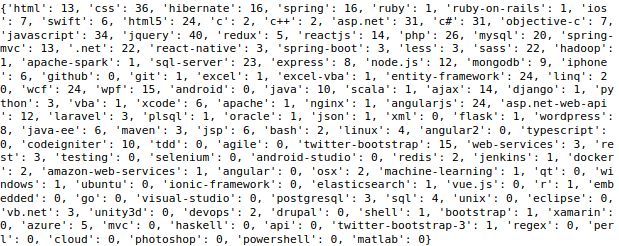
\includegraphics[width=10cm,height=5cm]{triangles}
			\caption{Network Triangles Networkx}
		\end{figure}
		\FloatBarrier
		For each node, the generalized degree shows how many edges of given triangle multiplicity the node is connected to. The triangle multiplicity of an edge is the number of triangles an edge participates in.
		\begin{figure}[ht]
			\centering
			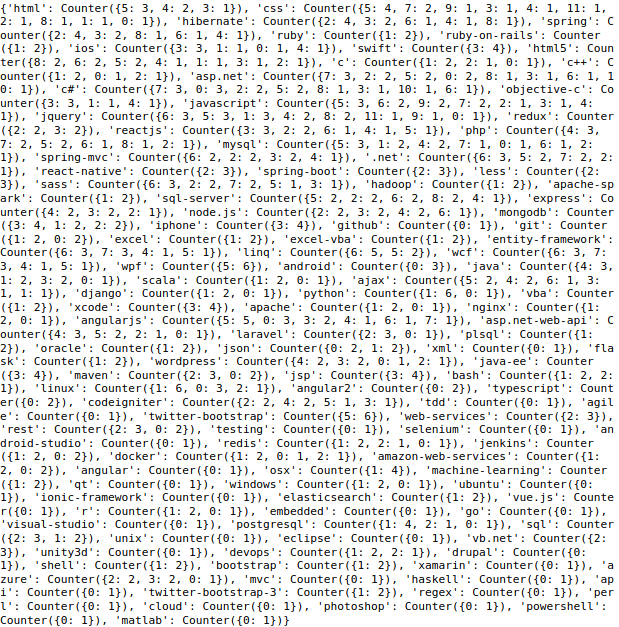
\includegraphics[width=10cm,height=9cm]{generalizeddegree}
			\caption{Generaliazed Degree}
		\end{figure}
		\FloatBarrier
		\section{Bridges}
			A bridge is a connection between two nodes that if it were to be deleted it would cause the total division of th main component into two separate components.
			\begin{figure}[ht]
				\centering
				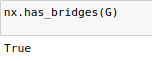
\includegraphics[width=3cm,height=1.5cm]{hasbridges}
				\caption{Networkx bridges}
			\end{figure}
			\FloatBarrier
			All the bridges of the network are the following:
			\begin{figure}[ht]
				\centering
				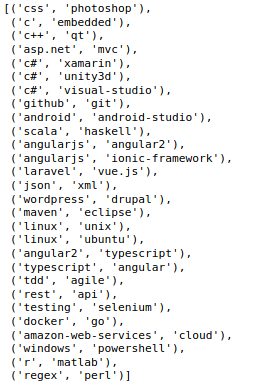
\includegraphics[width=6cm,height=8cm]{bridges}
				\caption{Generaliazed Degree}
			\end{figure}
			\FloatBarrier
		\section{Community}
			From the raw data there is the variable group, which is a result of clustering algorithm according to creators. Despite we already have an idea of communities, we run Modularity in Gephi and in networkx. This network has modularity 0.75 and we have 12 communities that correspond to a more specific prospect of groups.  
			\begin{figure}[ht]
				\centering
				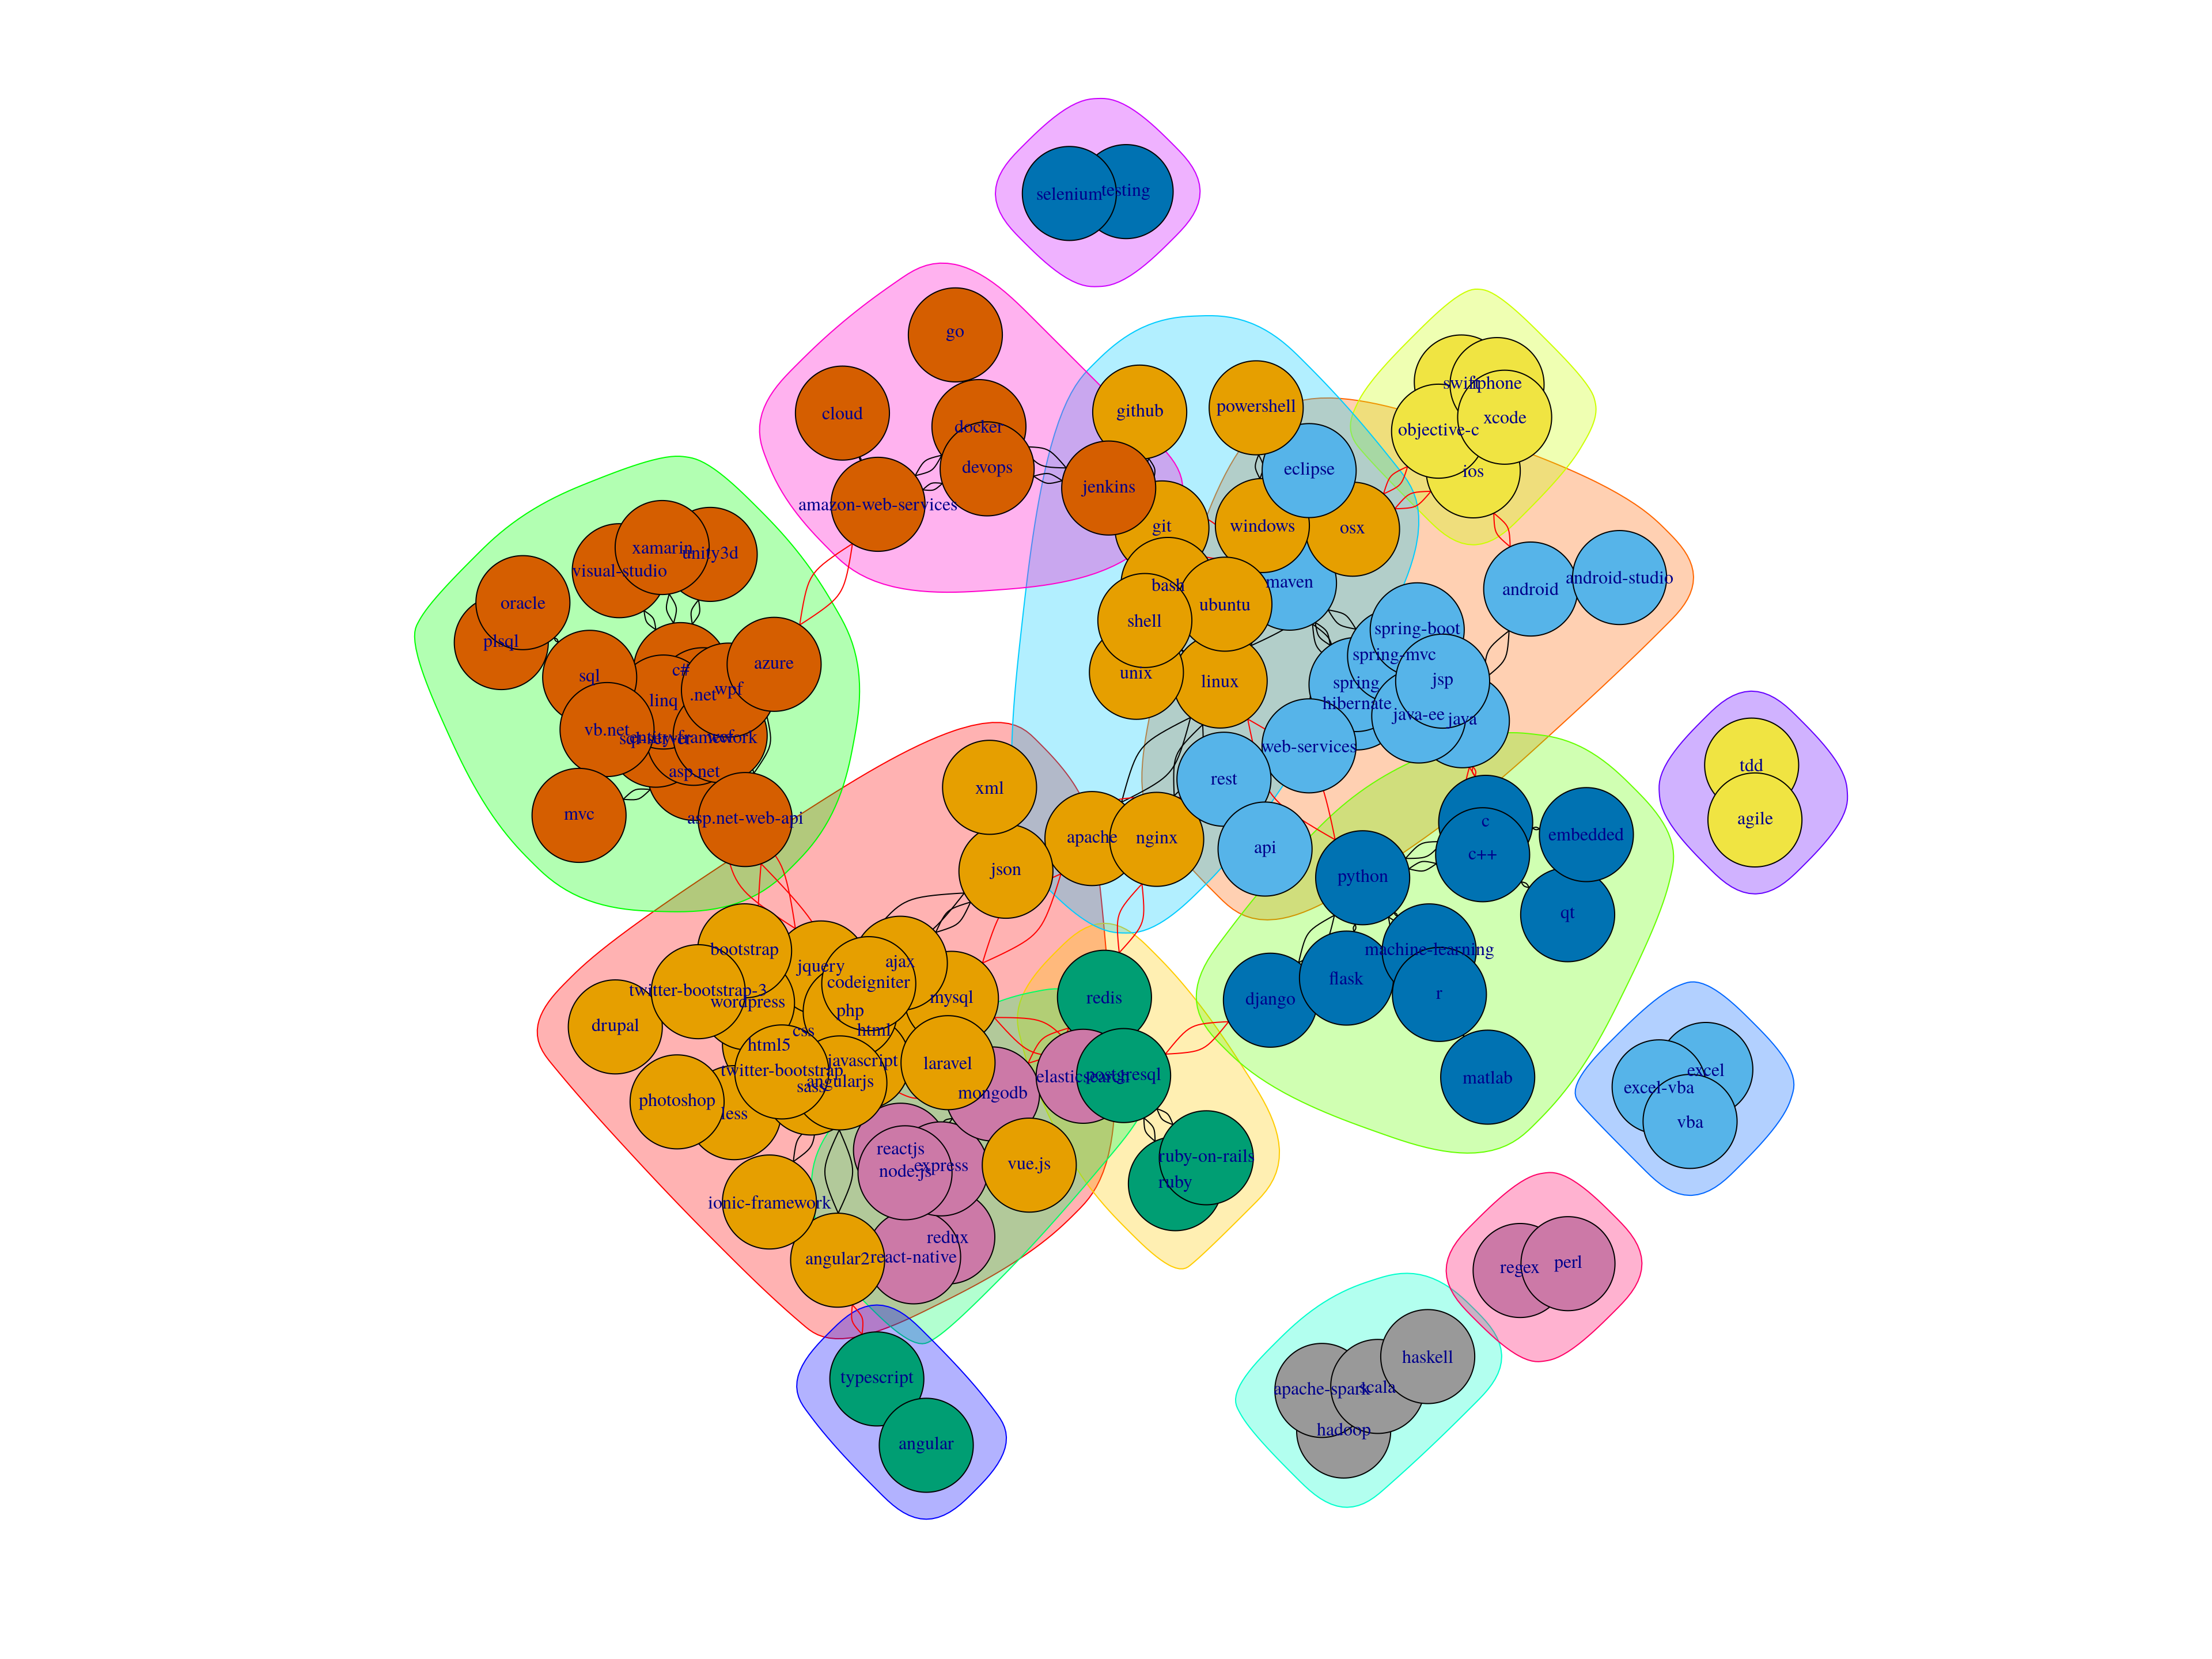
\includegraphics[width=16cm,height=15cm]{communities}
				\caption{Communities made with igraph}
			\end{figure}
			\FloatBarrier
			This graph is made with igraph and I found in this \href{https://www.kaggle.com/devisangeetha/network-visualizations-with-igraph}{source}.
			\subsection{Cliques}
				In general we consider cliques as groups of people who are closely connected to each other but not connected to people outside the group. In network theory a clique is defined as a maximal complete subgraph of a graph where each node is connected to all the other nodes. The word 'maximal' means that if we add another node to the clique the clique will cease to be a clique. nx.find\_cliques finds all the cliques in a network. We can also extract all the cliques from the tag network.\\
				The Stack Overflow tag network has 89 cliques according to networkx. 
			\subsection{Language Specific Subgraph And Cliques}
				For each programming language there's a tag in the network. E.g 'java' will refer to the Java Programming language. So we can check the cliques that contains that node. We can also visualize the subgraph containing that node and all its neighbours with a specified depth range.\\
				For example, we can check the ego network for Java with radius 2, which means that we get the subgraph containing Java and all it's direct neighbours which are 1 edge away from python and also the nodes which are 2 steps away from Java.\\
				These subgraphs called Ego networks and can be used for checking shortest paths or generally conducting analysis of who is connected to whom, but cliques are helpful because it shows us the data in a more granular way.\\
					\begin{figure}[ht]
						\centering
						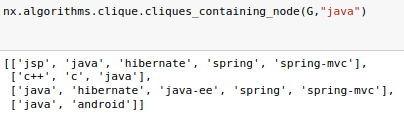
\includegraphics[width=9cm,height=3cm]{javacliq}
						\caption{Cliques including Java}
					\end{figure}
				\FloatBarrier
				Java participates in 4 different cliques, one for web development with jsp and sping-mvc, one for android development presumably which is connected to android. One for database management where it's adjacent to hibernate. Finally, the forth is more general acknowledgements, I presume, and Java is connected with C++ and C.
				\subsection{Max Cliques}
				 By using all the functions for cliques of Networkx project we conclude that the tags being includes in max cliques of this network are the followings:
				 \begin{enumerate}
				 	\begin{multicols}{3}
				 		\item .net
				 		\item ajax 
				 		\item asp.net 
				 		\item c\#
				 		\item css 
				 		\item entity-framework 
				 		\item javascript 
				 		\item jquery
				 		\item linq
				 		\item mysql 
				 		\item php 
				 		\item sql-server
				 		\item wcf
				 		\item wpf
				 	\end{multicols}
				 \end{enumerate}
			 We create a subgraph with 14 nodes, 43 edges and an average degree of $6.1429$. 
			 					\begin{figure}[ht]
			 	\centering
			 	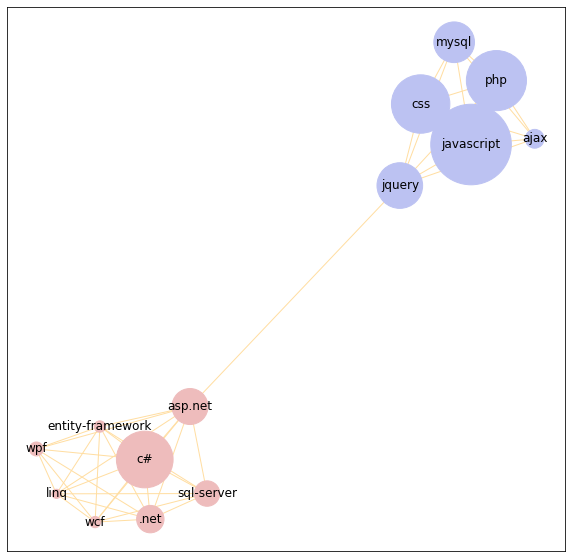
\includegraphics[width=12cm,height=11cm]{subgraph}
			 	\caption{Max Cliques Subgraph}
			 \end{figure}
			 \FloatBarrier
				 
				
		\section{Homophily}
			Homophily or Assortativity  is the tendency of individuals to choose friends with similar characteristic. “Like links with like.”
			The assortativity coefficient quantifies the extent to which connected nodes share similar  properties.  It  is  analogous  to  the  Pearson  correlation  coefficient  but measures  the  correlation  between  every  pair  of  nodes  that  are  connected. Depending  on  whether  the  node  property  of  interest  is  a  continuous  or  a categorical variable, there are two definitions of the assortativity coefficient.\\
			The current network which concerns technologies broadly used is absolutely natural not to enhance the phenomenon of homophily, due to the role of each technology-tag in the network. A typical example of that is the Linux  Operational System and Python Programming Language. There are connected, because all the applets in Linux are written in Python but Linux will never play a role of a programming language, so there is no case of choosing Python than Linux. They will always be complementary technologies. 
			\begin{figure}[ht]
				\centering
				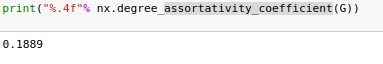
\includegraphics[width=9cm,height=1.5cm]{assortativity}
				\caption{Network's assortativity}
			\end{figure}
			\FloatBarrier
			The assortativity coefficient based on nodes' degree is calculated to be $0.19$. A  value close to 0 means no strong association of the property values between connected nodes. That is to say, the tags who are friend with each other tend to have different roles and significance in technology in general. \\
			The assortativity coefficient based on nodes' nodesize default variable is calculated to be $-0.0146$. A  value close to 0 means no strong association of the property values between connected nodes.\\
			\begin{figure}[ht]
				\centering
				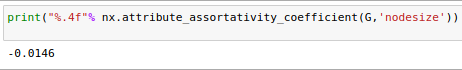
\includegraphics[width=9cm,height=1.5cm]{nodesizeassort}
				\caption{Network's assortativity based on nodesize}
			\end{figure}
			\FloatBarrier
			I also tried to visualize the homophily of the network by using the Axis Layout and by colouring each node according to the modularity class which belongs to. The result is the following impressing graph. If we combine the definition of homophily with the following graph, we may conclude that the nodes that are at the edges have the most negative assortativity coefficient and the other that are in the heart of that schema tend to have stronger association or recognition from the developers' community.
			\begin{figure}[ht]
				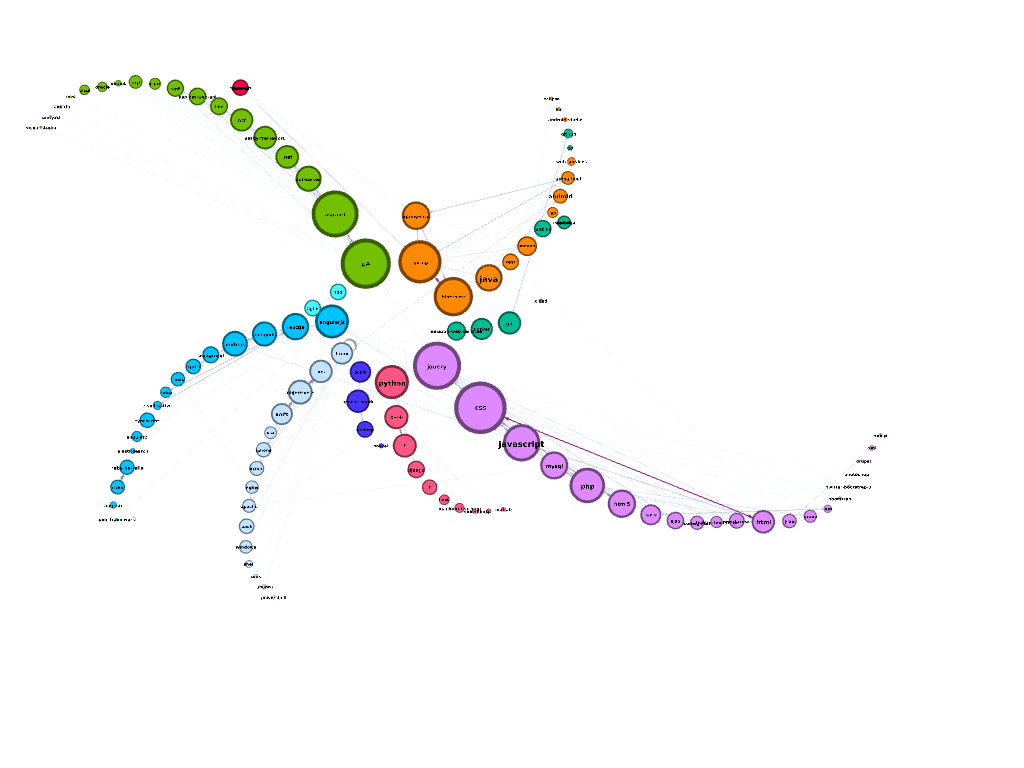
\includegraphics[width=21cm,height=18cm]{homophilymodclass}
				\caption{Network's assortativity based on modularity class}
			\end{figure}
			\FloatBarrier
			
		\section{Trends in Stack Overflow}
			I decided to visualise the most loved web frameworks as a network in order to answer one part of my initial questions "How to be up-to-date with current trending technologies? Which of them are perquisites of the others?". \\
			According to  \href{https://insights.stackoverflow.com/survey/2019#most-popular-technologies}{Stack Overflow Survey 2019} the most loved and wanted Web Frameworks are the following:
			\begin{enumerate}
				\begin{multicols}{2}
					\item reactjs
					\item vue.js 
					\item express 
					\item spring
					\item asp.net 
					\item django 
					\item flask 
					\item laravel 
					\item angularjs
					\item ruby-on-rails 
					\item jquery 
					\item drupal
				\end{multicols}
			\end{enumerate}
			\begin{figure}[ht]
				\centering
				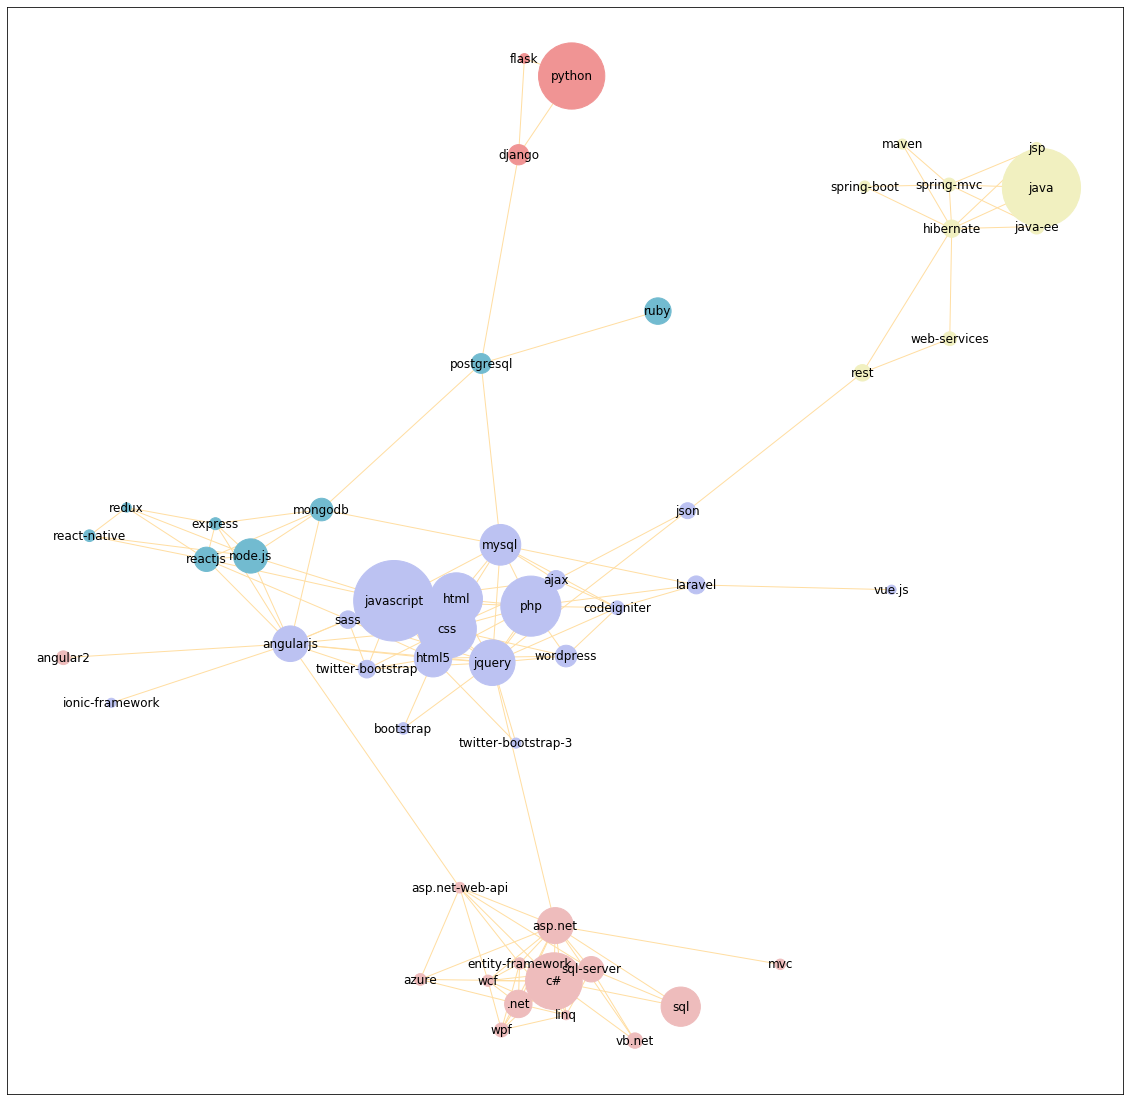
\includegraphics[width=15cm,height=15cm]{lovedplatforms}
				\caption{Most loved Web Frameworks network}
			\end{figure}
		\FloatBarrier
		As a result, I noticed that, for instance,  if one wants to become acquainted with JavaScript, he definitely should be first familiar with all of the javascript's tag neighbours (css, htl5, jquery etc.)
		
	\section{Conclusion}
		This network analysis confirms that technology trends are generally connected with one another. More specifically, it is proved that some technologies require some others in order to work effectively (e.g. jquery and html).
		On the other hand, there are technology that are completely independent, as for instance excel. This possibly means that either they are about to be extinct or they should change somehow in order to be compatible with others. 
		Last but not least, the current network analysis has compatible results with 2019 Trends Survey, highlighting that all widely used technologies have a lot in common as they may have a mutual starting node (e.g. Linux).

\begin{thebibliography}{9}

	\bibitem{barabasi} 
	 Barabási A.L 
	\textit{Network Science}. 
	Cambridge, United Kingdom: Cambridge University Press, 2012.
	
	\bibitem{easley} 
	Easley,D.,\& Kleinberg, J.
	\textit{Zur Elektrodynamik bewegter K{\"o}rper}. (German) 
	\textit{Networks, crowds, and markets}. 
	New York, NY: Cambridge University Press, 2010.
	
	\bibitem{lectures} 
	Lectures' Notes Prof. D. Pournarakis,
	\\\texttt{https://edu.dmst.aueb.gr/course/view.php?id=44}
	
	\bibitem{homphpres} 
	Naval Postgraduate School Monterey Homophily Presentation Prof. Ralucca Gera,
	\\\texttt{\href{https://faculty.nps.edu/rgera/MA4404/Winter2018/16-Homophily.pdf?fbclid=IwAR3rFajCl4mDfcfDCx6tLOanxDEX6k-p\_82etpYmmCSdmePeIMt-H7aZE2g}{Source}}
	
	\bibitem{networkx} 
	Networkx Documentation,
	\\\texttt{	https://networkx.github.io/documentation/stable/index.html}
	
	\bibitem{gephi} 
	Gephi Documentation,
	\\\texttt{https://gephi.org/users/}
	
	\bibitem{paper1} 
	Heba Elgazzar and Adel Elmaghraby,
	\textit{EVOLUTIONARY CENTRALITY AND MAXIMAL CLIQUES IN MOBILE SOCIAL NETWORKS}. 
	\\\texttt{https://arxiv.org/pdf/1809.02282.pdf}
	
	\bibitem{paper2} 
	Donglei Du,
	\textit{Social Network Analysis: Centrality Measures}
	\\\texttt{\href{http://www2.unb.ca/~ddu/6634/Lecture\_notes/Lecture\_4\_centrality\_measure.pdf}{Source}}
	
	\bibitem{pagerank} 
	Sage researchmethods datasets
	\textit{Learn About Assortativity Coefficient in Python With Data From UK Faculty Dataset}
	\\\texttt{\href{https://methods.sagepub.com/base/download/DatasetStudentGuide/assortativity-in-ukfaculty-2008-python}{Source}}
	
	\bibitem{dataanalysispython} 
    John Ladd, Jessica Otis, Christopher N. Warren, and Scott Weingart,
	\textit{Exploring and Analyzing Network Data with Python }. 
	\\\texttt{\href{https://programminghistorian.org/en/lessons/exploring-and-analyzing-network-data-with-python}{Source}}
	
	\bibitem{networkxrepo1} 
	Tutorial Repository by 	Mridul Seth,
	\\\texttt{https://github.com/MridulS/pydata-networkx}
	
	\bibitem{networkxrepo2} 
	Tutorial Repository for Networkx,
	\\\texttt{https://github.com/networkx}
	
	\bibitem{tutorialytb} 
	Tutorial Video to import .csv in Gephi,
	\\\texttt{	\href{https://www.youtube.com/watch?v=HJ4Hcq3YX4k\&feature=youtu.be\&fbclid=IwAR2MaJUsRRWxwagv2bRxdKOqcozzb4fDDgM9qpPTLrsVLpwq8ycb1aaW7mU}{Source}}
\end{thebibliography}


\end{document}